\section{Prima Parte}

\subsection{Implementazione DCT2}

La nostra implementazione di DCT 2D prevede principalmente 2 passi: la computazione della matrice D per la Discrete Cosine Transform e la dct2, costituita dall'esecuzione prima sulle colonne e poi sulle righe della matrice da trasformare, della dct monodimensionale, facendo uso della matrice D.

\lstinputlisting[language=Python]{CODE/Part1/compute_D.py}

Oltre alla DCT bidimensionale, riportata di seguito, è stata anche implementata la DCT monodimensionale, e le rispettive inverse per entrambe, di cui si omette il codice per brevità.

\lstinputlisting[language=Python]{CODE/Part1/my_dct2.py}

Trattandosi di un'implementazione molto semplificata, senza particolari ottimizzazioni, non ci si aspetta grandi risultati in termini di efficienza, con una complessità computazionale asintotica attesa nell'ordine di $\mathcal{O}(n^3)$

\subsection{La libreria dctn}
% implementa sia dctn che idctn con FFT, quindi ci aspettiamo n^2log(n)
% parametro norm=ortho per ottenere risultati come sul pdf

Passando all'implementazione open source, avendo scelto Python quale linguaggio di programmazione, la scelta della libreria è virata su \textit{scipy.fftpack}, che implementa sia la \textit{dct} monodimensionale, che la \textit{dctn}, bidimensionale, entrambe con le rispettive inverse.

La libreria inoltre lavora per mezzo della \textit{FFT}, Fast Fourier Transform, pertanto i risultati attesi sono migliore della nostra implementazione descritta in precedenza, con una complessità computazionale asintotica attesa nell'ordine di $\mathcal{O}(n^2\log{}n)$

\subsection{Verifica dello Scaling}

Nel dettaglio la libreria offre inoltre diversi paramentri personalizzabili, su tutti i 4 diversi tipi di implementazione di dct, oltre a 3 differenti norme per il calcolo.\\
Di queste ultime, la norma utilizzata di default dalla libreria è la \textit{backward}, i cui risultati non coincidevano con quelli visti a lezione. Per ottenre lo stesso scaling, necessario per la seconda parte del progetto, è bastato modificare il parametro a \textit{ortho}, per ottenere scaling ortogonale

\subsection{Analisi Sperimentale dei Risultati}
% elenca valori di N utilizzati
% parametro per idctn = 0.5
Punto focale della prima parte del progetto è stato quello dell'analisi dei risultati delle due implementazioni di DCT, per confrontarne i risultati in termini di efficienza computazionale.

Nello specifico sono stati fatti test ripetuti, iternado su matrici di dimensioni che vanno a partire da \textit{N=8} a \textit{N=10.000}, ed eseguendo su di esse entrmabe le implementazioni di \textit{DCT-2D}, misurandone i tempi di esecuzione, e sui 2 risultati ottenuti, le rispettive DCT inverse.

Di seguito è mostrato il pattern di creazione delle matrice testate, che è lo stesso visto a lezione. La scelta di avere un pattern definito per tutte le matrici, anche al crescere delle dimesioni, può essere motivata dal fatto che volendo effetturare un'analisi quanto più possibile precisa e rappresentativa dei risultati, abbiamo preferito evitare di inserire una componente randomica all'interno del processo

\lstinputlisting[language=Python]{CODE/Part1/matrix_pattern.py}

Un esempio di matrice costruita in questo modo attraverso il parametro \textit{N=8} è il seguente

\[
\begin{matrix}
       1  &       1  &       1  &       1  &     -1  &     -1  &     -1  &     -1 \\
       1  &       1  &       1  &       1  &     -1  &     -1  &     -1  &     -1 \\
       1  &       1  &       1  &       1  &     -1  &     -1  &     -1  &     -1 \\
       1  &       1  &       1  &       1  &     -1  &     -1  &     -1  &     -1 \\
     -1  &     -1  &     -1  &     -1  &       1  &       1  &       1  &       1 \\
     -1  &     -1  &     -1  &     -1  &       1  &       1  &       1  &       1 \\
     -1  &     -1  &     -1  &     -1  &       1  &       1  &       1  &       1 \\
     -1  &     -1  &     -1  &     -1  &       1  &       1  &       1  &       1
\end{matrix}
\]

I risultati ottenuti sono dunque mostrati nella tabella \ref{tab:dct_times}, suddivisi per algoritmo applicato e dimensione della matrice.\\
Si nota subito come le esecuzioni più pesanti abbiano impiegato tempi considerevoli, soprattuto per l'implementazione fatta da noi, in particolare per \textit{N=10.000}, il cui tempo complessivo di esecuzione è stato di 53 minuti, mentre l'intera esecuzione ha richiesto 2 ore e 45 minuti totali.

% dataset risultati
\begin{table}[H]
    \centering
    \scalebox{1}{
\begin{tabular}{rrrrr}
\toprule
      N &     my\_dct2 &  scipy\_dct2 &    my\_idct2 &  scipy\_idct2 \\
\midrule
    8.0 &    0.000000 &    0.000958 &    0.000000 &     0.000000 \\
   16.0 &    0.000000 &    0.000000 &    0.002004 &     0.000000 \\
   32.0 &    0.003052 &    0.000000 &    0.001994 &     0.000000 \\
   64.0 &    0.016999 &    0.000000 &    0.040002 &     0.000000 \\
  100.0 &    0.048003 &    0.000995 &    0.038997 &     0.001000 \\
  250.0 &    0.171372 &    0.001997 &    0.191005 &     0.000997 \\
  500.0 &    0.585959 &    0.009003 &    0.728988 &     0.003996 \\
  750.0 &    1.757999 &    0.017997 &    1.682003 &     0.016996 \\
 1000.0 &    3.473949 &    0.041000 &    4.368999 &     0.029999 \\
 1500.0 &    8.694001 &    0.079000 &   10.939000 &     0.073998 \\
 2000.0 &   17.948997 &    0.140060 &   22.092954 &     0.169000 \\
 2500.0 &   33.305009 &    0.238048 &   34.149954 &     0.311993 \\
 3000.0 &   54.187999 &    0.512000 &   56.753988 &     0.408993 \\
 3500.0 &   80.074001 &    0.511000 &   90.720990 &     0.604976 \\
 4000.0 &  112.808998 &    0.641059 &  128.283914 &     0.608915 \\
 4500.0 &  151.504001 &    0.851001 &  149.634990 &     0.964912 \\
 5000.0 &  198.861000 &    1.153052 &  199.803908 &     1.216013 \\
 6000.0 &  324.213001 &    1.609000 &  319.287986 &     1.787985 \\
 7000.0 &  528.754846 &    2.923000 &  514.121990 &     2.724993 \\
 8000.0 &  733.791951 &    3.921043 &  742.012907 &     3.891963 \\
 9000.0 & 1053.912169 &    4.901043 & 1098.505610 &     4.820091 \\
10000.0 & 1550.146987 &    5.979995 & 1631.578991 &     7.541971 \\
\bottomrule
\end{tabular}
}
    \caption{DCT Times}
    \label{tab:dct_times}
\end{table}

% grafici Jupyter da commentare
    % da evidenziare la forma di distribuzione attesa uguale a quella ottenuta
\subsection{DCT comparison}

Si parte dal confronto della \textit{DCT2} implementata con quella della libreria \textit{scipy}.\\
Le figure \ref{fig:dct2_comparison} e \ref{fig:dct2_log_comparison} mostrano i tempi di esecuzione al crescere della dimensione della matrice.

Oltre ai tempi di esecuzione, sono stati tracciate sul grafico anche le forme delle funzioni $n^{3}$ e $n^{2}\log{}n$, divise per un coefficiente di normalizzazione per fare in modo che solo l'ultimo valore coincidesse con i tempi effettivi.\\
Si nota come in entrambi i casi le funzioni assumano la forma attesa, se non per alcune differenze negli stadi di osservazione iniziali.

\begin{figure}[H]
\hspace*{-2cm} 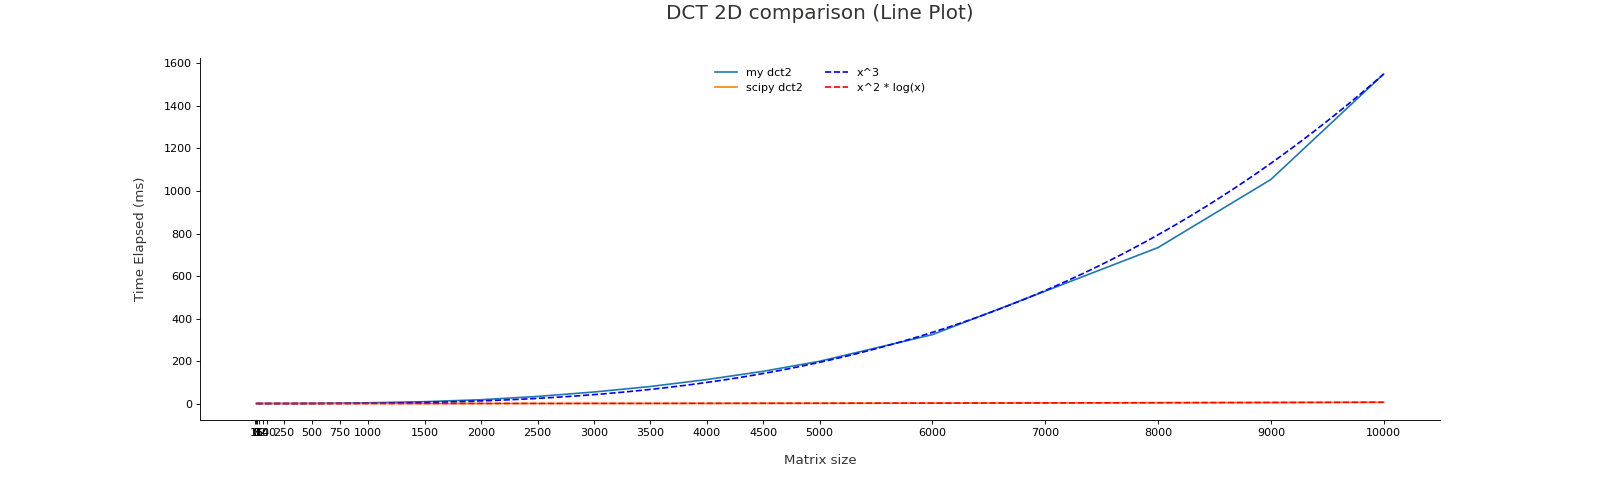
\includegraphics[scale=0.4]{figs/DCT Comparison/dct2_comparison.png}
    \caption{DCT2 comparison}
    \label{fig:dct2_comparison}
\end{figure}

\begin{figure}[H]
\hspace*{-2cm} 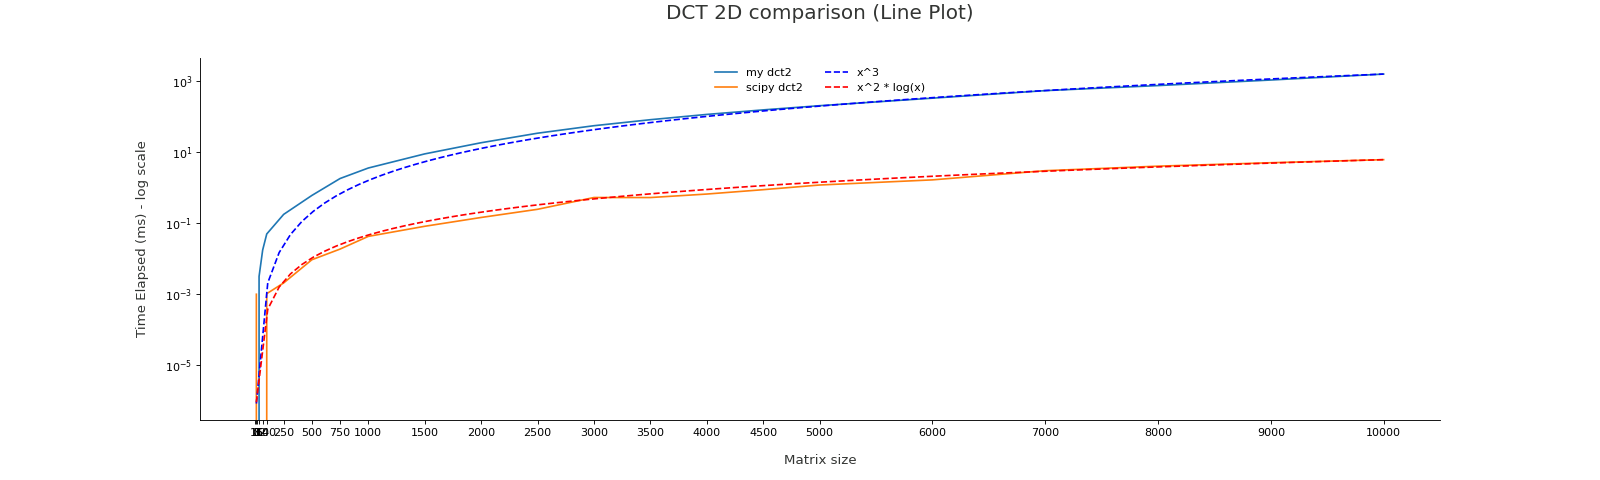
\includegraphics[scale=0.4]{figs/DCT Comparison/dct2_log_comparison.png}
    \caption{DCT2 semi-log comparison}
    \label{fig:dct2_log_comparison}
\end{figure}

\subsection{iDCT comparison}

Lo stesso paragone è stato fatto per le \textit{inverse-DCT 2D}, confrontando la nostra implementazione con quella di \textit{scipy}.

I risultati mostrati nelle figure \ref{fig:idct2_comparison} e \ref{fig:idct2_log_comparison} seguono la stessa tendenza di quelli visti per \textit{DCT2}.\\
Anche in questo caso la forma assunta dal grafico dei risultati segue precisamente quella della funzione attesa.

\begin{figure}[H]
\hspace*{-2cm} 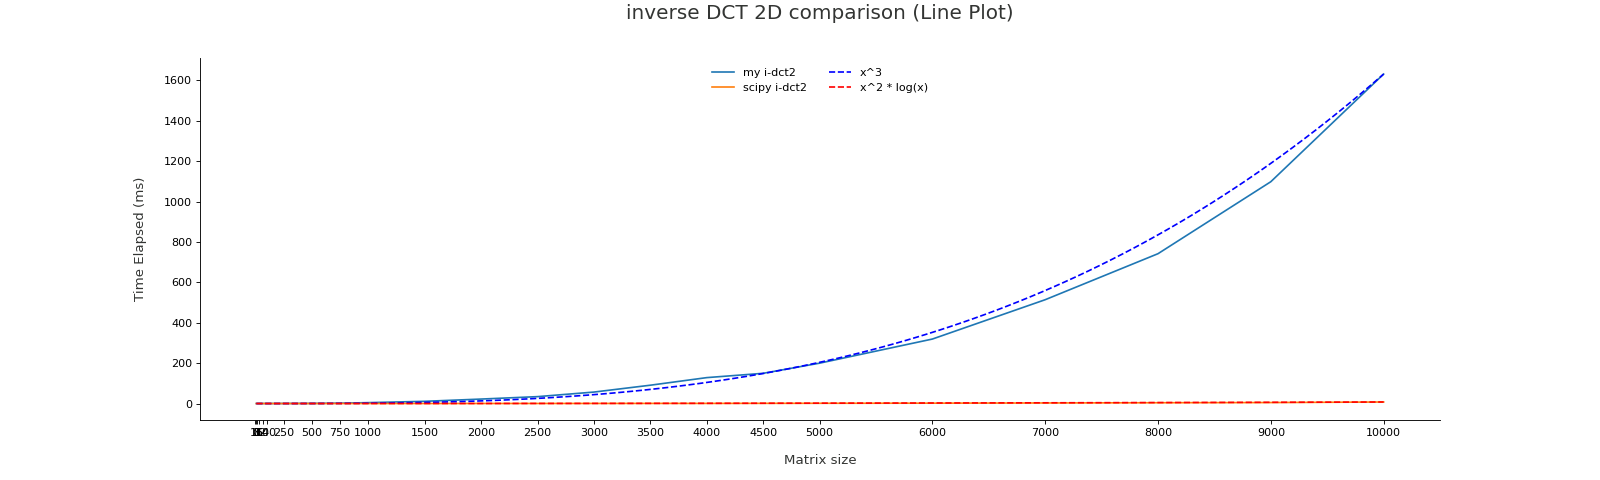
\includegraphics[scale=0.4]{figs/DCT Comparison/idct2_comparison.png}
    \caption{inverse DCT2 comparison}
    \label{fig:idct2_comparison}
\end{figure}

\begin{figure}[H]
\hspace*{-2cm} 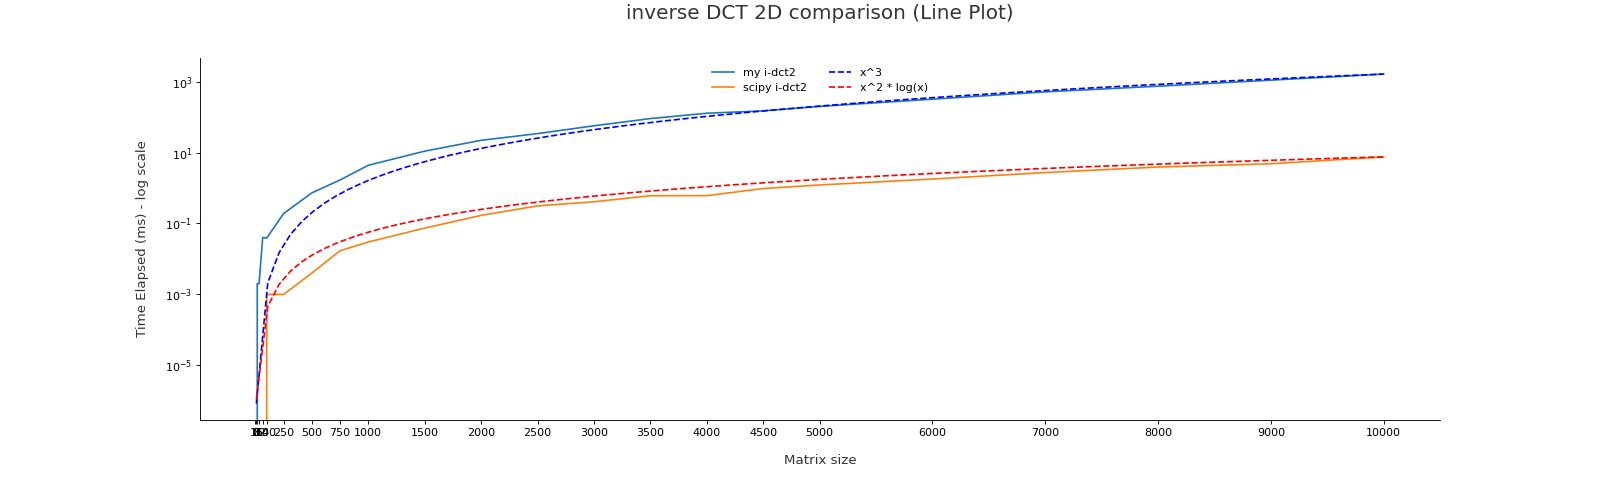
\includegraphics[scale=0.4]{figs/DCT Comparison/idct2_log_comparison.png}
    \caption{inverse DCT2 semi-log comparison}
    \label{fig:idct2_log_comparison}
\end{figure}

\subsection{DCT vs iDCT}

Un'ultima breve analisi eseguita è stata quella per confrontare la nostra le \textit{DCT2} e le \textit{iDCT2} delle rispettive implementazioni tra di loro.

La figura \ref{fig:my_dcts_log_comparison} mostra come le differenze tra le due funzioni siano praticamente nulle, con la \textit{DCT2} che in media impiega \textit{6 secondi} in meno della \textit{iDCT2}, con una differenza massima di \textit{81 secondi} per \textit{N=10.000}.\\
Tuttavia in alcuni casi la \textit{iDCT} risulta addirittura più veloce della sua controparte, nonostante il suo calcolo richieda il calcolo dell'inversa della matrice da trasformare

\begin{figure}[H]
\hspace*{-2cm} 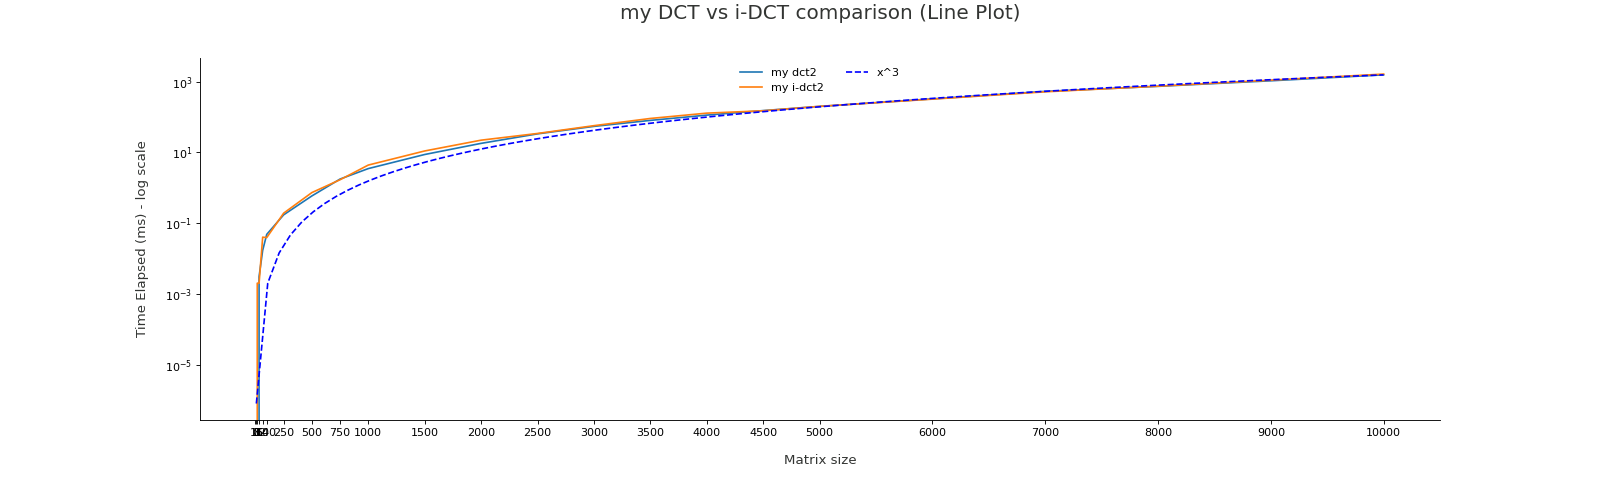
\includegraphics[scale=0.4]{figs/DCT Comparison/my_dcts_log_comparison.png}
    \caption{my DCTs semi-log comparison}
    \label{fig:my_dcts_log_comparison}
\end{figure}

Anche per l'implementazione delle funzioni in \textit{scipy} la tendenza è la stessa. Qui troviamo che in media \textit{DCT2} impiega \textit{0.075 secondi} in meno, con un picco di \textit{1.5 secondi} di vantaggio per \textit{N=10.000}.\\

\begin{figure}[H]
\hspace*{-2cm} 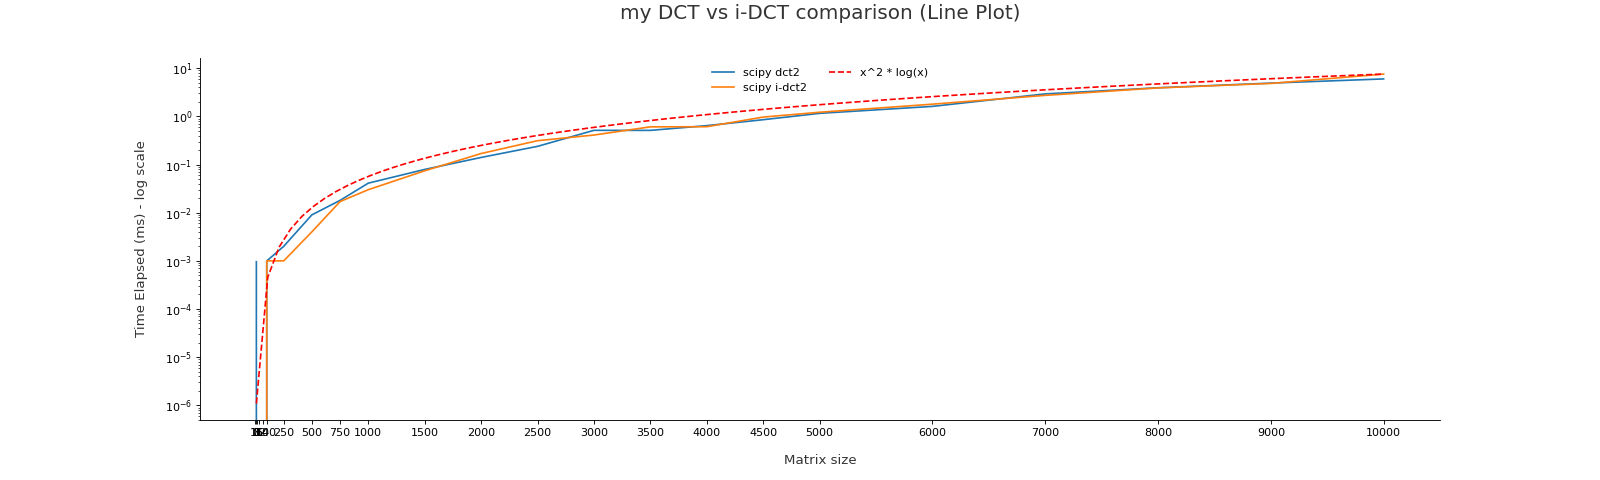
\includegraphics[scale=0.4]{figs/DCT Comparison/scipy_dcts_log_comparison.png}
    \caption{scipy DCTs semi-log comparison}
    \label{fig:scipy_dcts_log_comparison}
\end{figure}